\begin{figure}[tp]
	\centering
	\begin{lrbox}{\mintedbox}
		\begin{minipage}{0.48\textwidth}
			\tscode{code/background/typescript/declaration-files/calculator-index.d.ts}
		\end{minipage}
	\end{lrbox}
	\subfloat[calculator/index.d.ts]{\usebox{\mintedbox}}
	\hfill
	\begin{lrbox}{\mintedbox}
		\begin{minipage}{0.48\textwidth}
			\jscode{code/background/typescript/declaration-files/calculator-index.js}
		\end{minipage}
	\end{lrbox}
	\subfloat[calculator/index.js]{\usebox{\mintedbox}}

	\subfloat[Visual Studio Code auto-completion]{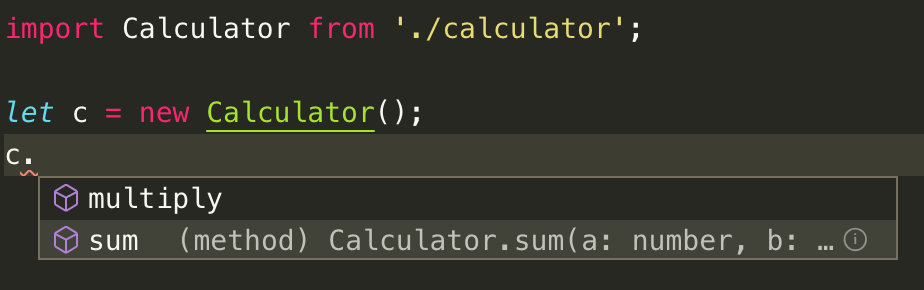
\includegraphics[width=0.7\textwidth]{figures/background/typescript/declaration-files/ide-auto-completion.png}}

	\begin{lrbox}{\mintedbox}
		\begin{minipage}{0.58\textwidth}
			\jscode{code/background/typescript/declaration-files/index.ts}
		\end{minipage}
	\end{lrbox}
	\subfloat[index.ts]{\usebox{\mintedbox}}
	\hfill
	\begin{lrbox}{\mintedbox}
		\begin{minipage}{0.4\textwidth}
			\begin{bashinline}
$ tsc index.ts
$ node index.js
Computing [(1+2) * (3+4)] ...
The result is: 21
			\end{bashinline}
		\end{minipage}
	\end{lrbox}
	\subfloat[Console output]{\usebox{\mintedbox}}

	\caption[TypeScript declaration files]{\textbf{TypeScript declaration files} - A TypeScript project using the declaration file of an external JavaScript library \mintinline{text}{calculator}. IDE auto-completion and compiler make use of the declaration file.}
	\label{fig:background-declaration-files-calculator-example}
\end{figure}